\section{Analysis}
\label{sec:Analysis}

\subsection{Kinematics of the simulated data}
\label{sec:simdata}
To get to know the underlying process, the data simulated by Monte Carlo is analysed for its kinetic properties. The vector components of the momentum
of one of the hadrons is shown in \autoref{fig:P_H1XYZ}. The momentum in the x- and y- direction follow a gaussian distribution. These two axes are perpendicular
to the beam. However, the z-component shows negative exponential behaviour.
\begin{figure}
  \centering
  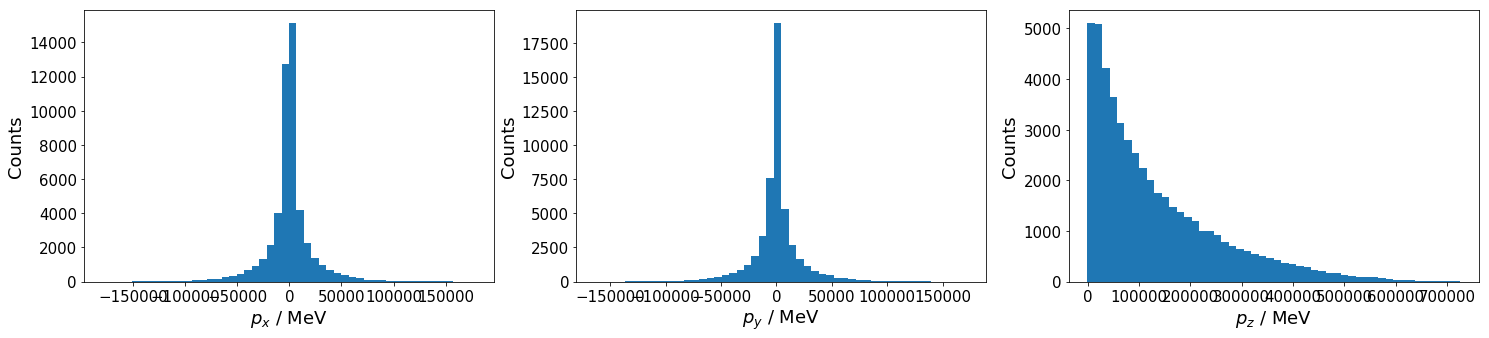
\includegraphics[width = .95\textwidth]{"content/pics/P_H1XYZ.png"}

  \caption{Histograms of the distributions of the momentum vector components for the first hadron of the simulated data.}
  \label{fig:P_H1XYZ}
\end{figure}
\\ With these quantities, the magnitude of the momentum can be calculated via 
\begin{equation}
  \label{eq:magn_p}
    p = \sqrt{p_x^2 + p_y^2 + p_z^2}.
\end{equation}
This is done for every kaon candidate and every event.
The resulting distribution of the magnitude of the momentum is shown in \autoref{fig:P_H1}.
\begin{figure}
  \centering
  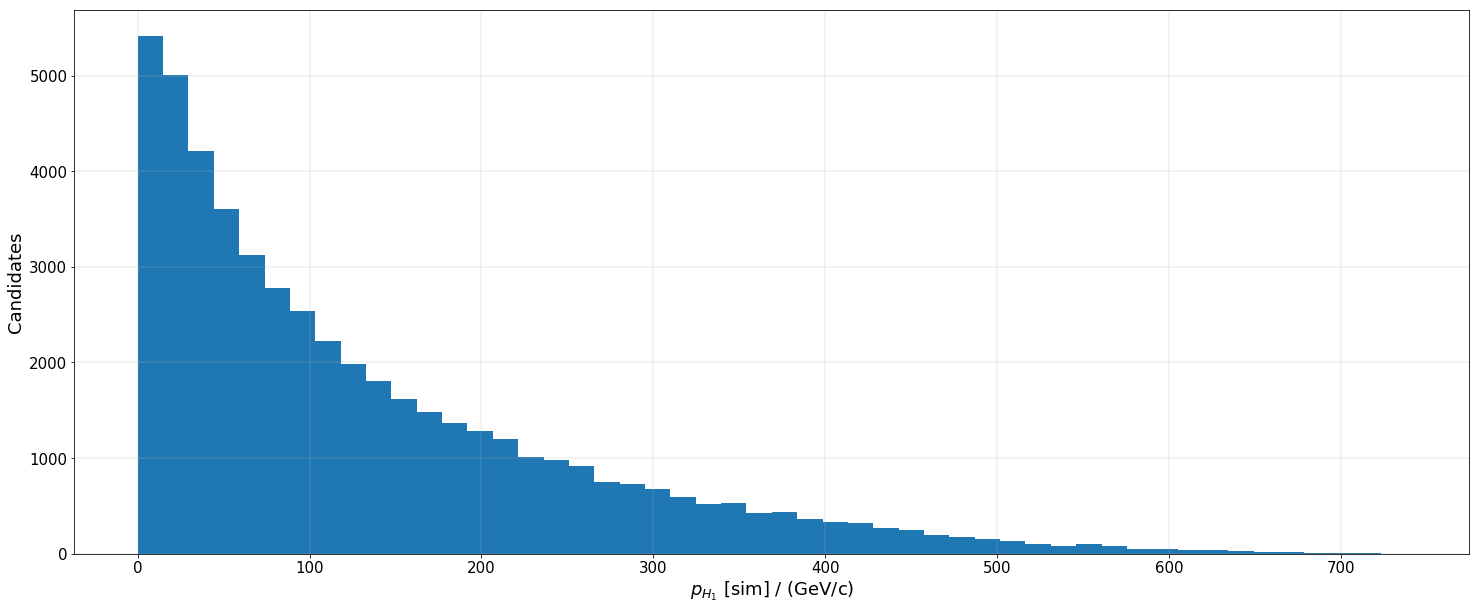
\includegraphics[width = .95\textwidth]{"content/pics/P_H1.png"}
  \caption{Histogram of the magnitude of the momentum for the first hadron of the simulated data.}
  \label{fig:P_H1}
\end{figure}
\\ By using the realtion of energy, mass and momentum \autoref{eq:energy-momentum-mass}, the energy of the hadrons can be calculated. The kaon mass is well known and documented by the Particle Data Group \cite{PDG}.
It is given by $m_{K^{\pm}} = \qty{493.677(0.015)}{\mega\electronvolt}$. The resulting energy distribution of the first hadron is depicted in  \autoref{fig:E_H1}.
\begin{figure}
  \centering
  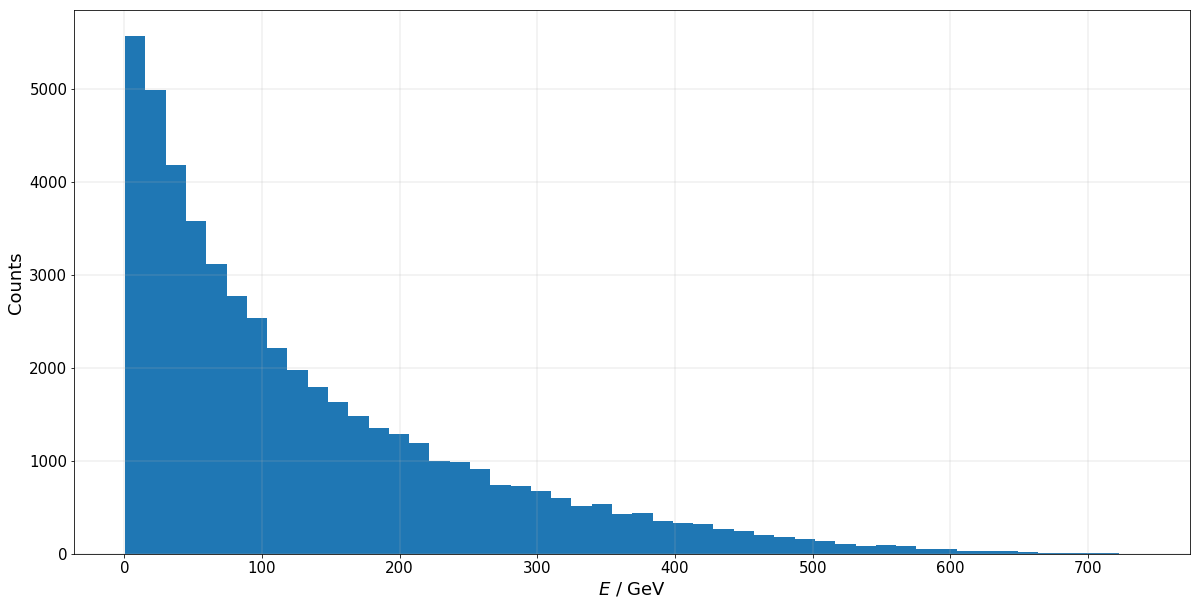
\includegraphics[width = .95\textwidth]{"content/pics/E_H1.png"}
  \caption{Histogram of the energy of the first hadron of the simulated data.}
  \label{fig:E_H1}
\end{figure}
\\The energy is also calculated for the other kaon candidates. Since energy and momentum is a conserved quantity, the energy and momentum of the $B^{\pm}$ meson can be calculated
using the energy and momentum of the three kaon candidates. The single momentum components of all final state particles are added together and the magnitude of the momentum of the $B^{\pm}$
meson can be calculated via \autoref{eq:magn_p}. The energy is calculated by summing the energy of all final state particles. With the energy and the magnitude of the momentum, the resulting
mass of the $B^{\pm}$ meson can be calculated via \autoref{eq:energy-momentum-mass}. The resulting distribution can be seen in \autoref{fig:B_M_sim}.
\begin{figure}
  \centering
  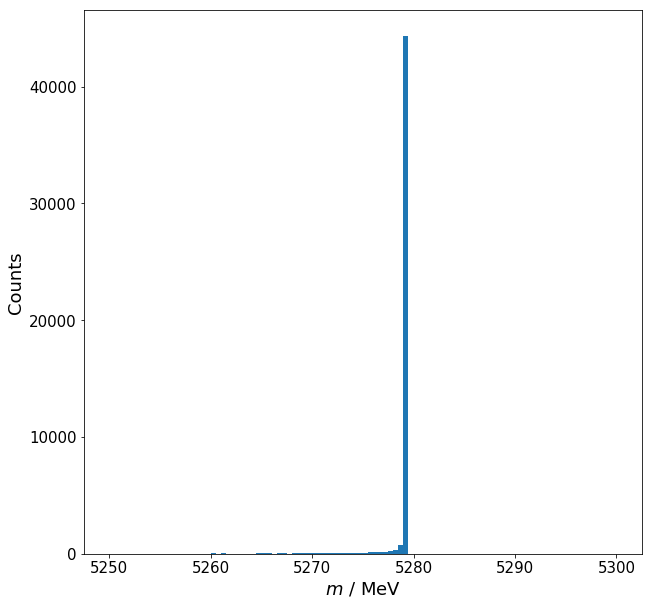
\includegraphics[width = .95\textwidth]{"content/pics/B_M_sim.png"}
  \caption{Histogram of the mass of the $B^{\pm}$ meson of the simulated data.}
  \label{fig:B_M_sim}
\end{figure}
The distribution has a sharp peak at the mass of the $B^{\pm}$ meson ($m_{B^{\pm}} = \qty{5279.41(0.07)}{\mega\electronvolt}$ \cite{PDG}). This is due to the fact, that this is simulated data using information about the mass of the $B^{\pm}$ meson during
the simulation process. The distribution for real data would a lot broader and will also contain combinatorial background.

\subsection{Preselection}

To reduce combinatorial background and misidentified decays as well as selecting only the decay into kaons, tighter cuts on the given parameters are needed. By using the distributions of the given
parameters (\autoref{fig:ProbKPi}), that describe the likeliness of the hadron being a specific particle, one can decide for appropriate cuts. This is done for all three final state
hadrons. When choosing the cut, it is wise to not cut too tight. This would reduce signal events and worsen the statistics. Also, to ensure that the
hadrons are not muons, the variable \texttt{isMuon} is used for the preselection. The chosen cuts are listed
in \autoref{tab:Preselection}.
\begin{table}[h!]
  \centering
    \begin{tabular}{ |p{3cm}||p{3cm}|p{3cm}|p{3cm}|  }
      \hline
      \multicolumn{4}{|c|}{Preselection} \\
      \hline
      Variable & Hadron 1 &Hadron 2 &Hadron 3\\
      \hline
      \texttt{isMuon} (boolean)   & is not &is not&  is not\\
      \texttt{ProbK}&   $> 0.6$  &$> 0.55$   &$> 0.85$\\
      \texttt{ProbPi} & $< 0.3$ & $< 0.3$&  $< 0.3$\\
      \hline   
    \end{tabular}
    \caption{The chosen cuts for the preselection of the recorded data. The values are chosen according to the distributions shown in \autoref{fig:ProbKPi}.}
    \label{tab:Preselection}
\end{table}
\begin{figure}
  \centering
  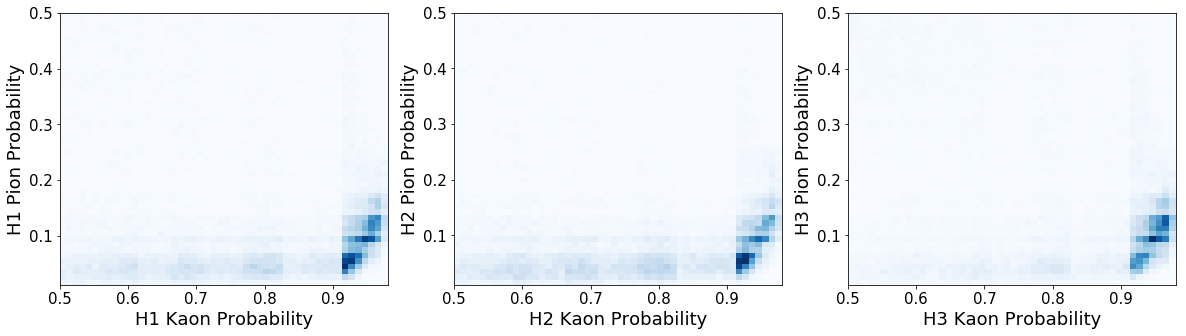
\includegraphics[width = .95\textwidth]{"content/pics/ProbKPi.png"}

  \caption{A 2-dimensional histogram for the Kaon and Pion Probability of the three hadrons.}
  \label{fig:ProbKPi}
\end{figure}
The magnitude of the momentum, the energy as well as the mass of the $B^{\pm}$ meson is calculated for the real data, just like it has been done in \autoref{sec:simdata} for the simulated data.
The resulting distribution of the $B^{\pm}$ meson mass can be seen in \autoref{fig:B_M_real}.
\begin{figure}
  \centering
  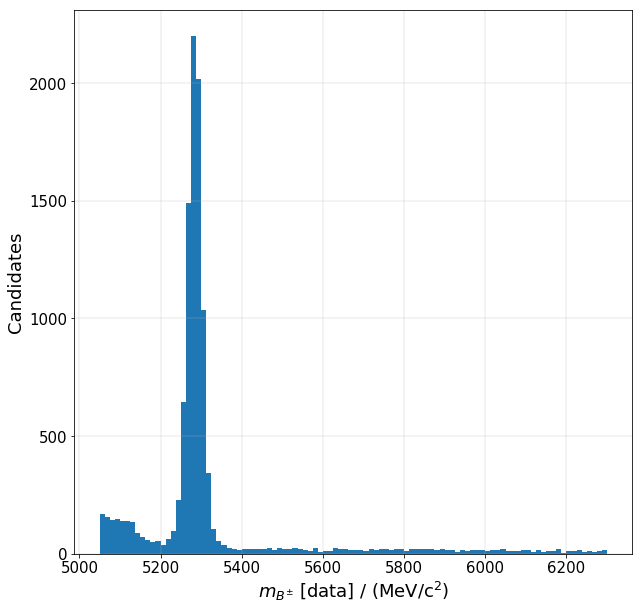
\includegraphics[width = .95\textwidth]{"content/pics/B_M_real.png"}
  \caption{Histogram of the mass of the $B^{\pm}$ meson of the recorded data.}
  \label{fig:B_M_real}
\end{figure}
\\ The gaussian distribution of the mass of the $B^{\pm}$ meson is much broader and also contains uniform background as well as a more dominant background on the lower end of the invariant mass.
To reject the background further, a cut on the $B^{\pm}$ meson mass is applied as $m_B > \qty{5200}{\mega\electronvolt}$ and $m_B < \qty{5400}{\mega\electronvolt}$. Multiple 
cuts are tested. The chosen cuts seem to be the best choice for rejected most background, while maintaining much signal.\\

\subsection{global matter anti-matter differences}

To study possible CP violation, the dataset has to be splited for events with $B^+ \rightarrow K^+ K^+ K^-$ and $B^- \rightarrow K^- K^+ K^-$. The $B^{\pm}$ meson charge is established by 
looking at the charge of the kaon candidates. Those events, which have two negatively charge kaons came from a $B^-$ meson and those with two positively charged kaons from a $B^+$ meson.
The asymmetry is the calculated by summing the number of events in each dataset and using
\begin{equation}
  A_{CP} = \frac{N^+ - N^-}{N^+ + N^-}.
\end{equation}
The resulting global asymmetry for the selected events is $A_{CP} = 0.0436$. In particle physics, a value is only considered an observation, if it is at least five standard deviations. If it exceeds
three sigma, it is considered evidence. The uncertainty of the asymmetry can be calculated via
\begin{equation}
  \label{eq:unc}
  \sigma_A = \sqrt{\frac{1-A_{CP}^2}{N^+ + N^-}}.
\end{equation}
The significance is the asymmetry devided by the resulting uncertainty. The uncertainty for the selected events is $\sigma_A = 0.0109$ and the significance is $S = 4.0041$. The calculated asymmetry can therefore be regarded 
as evidence.\\
However, the statistical uncertainty is not the only uncertainty that should be regarded when analysing this decay. The production asymmetry can be approximated with $1\%$. By using \autoref{eq:unc}, the uncertainty
for the production asymmetry is $\sigma_P = 0.0109$. Using gaussian error propagation, the final uncertainty is $\sigma_{All} = 0.0154$ and the significance therefore $S = 2.8300$. The result is therefore
no longer regarded as evidence.

\subsection{Dalitz plots and resonances}

\subsection{Local matter anti-matter differences}